\documentclass[11pt,onecolumn,a4paper]{article}

\usepackage{geometry}
 \geometry{
 a4paper,
 total={210mm,297mm},
 left=20mm,
 right=20mm,
 top=20mm,
 bottom=20mm,
 }
\usepackage{times}
\usepackage{epsfig}
\usepackage{epstopdf}
\usepackage{graphicx}
\usepackage{amsmath}
\usepackage{amssymb}
\usepackage{listings}
\usepackage{url}
\usepackage[english]{babel}

% Include other packages here, before hyperref.

% If you comment hyperref and then uncomment it, you should delete
% egpaper.aux before re-running latex.  (Or just hit 'q' on the first latex
% run, let it finish, and you should be clear).
%\usepackage[pagebackref=true,breaklinks=true,letterpaper=true,colorlinks,bookmarks=false]{hyperref}


\begin{document}

%%%%%%%%% TITLE
\title{Evolutionary Feature Selection}

\author{Thomas Bergmueller\\
Authentic Vision, University of Salzburg\\
Salzburg, Austria\\
{\tt\small tb@authenticvision.com}
% For a paper whose authors are all at the same institution,
% omit the following lines up until the closing ``}''.
% Additional authors and addresses can be added with ``\and'',
% just like the second author.
% To save space, use either the email address or home page, not both
\and
Eleftherios Christopoulos, Martin Schnoell\\
University of Salzburg\\
Salzburg, Austria\\
{\tt\small \{martin.schnoell, eleftherios.christopoulos\}@stud.sbg.ac.at}
}



\maketitle
\thispagestyle{empty}
\newpage
%%%%%%%%% ABSTRACT
\begin{abstract}
   In this paper the main goal was to identify the best feature subset that provides the highest accuracy for every dataset with the use of Evolutionary Algorithms. Since for every large dataset checking all possible feature subsets cannot be done in reasonable computation time. Also an evaluation of the parameters affecting the accuracy is presented.
\end{abstract}
\newpage
%%%%%%%%% BODY TEXT
\section{Introduction}
\label{l}
An Evolutionary Algorithm (EA) belongs to the spectrum of evolutionary computation. EAs differentiate themselves from traditional methods due to their search for a solution from a population and not from a single point. They are often used for non-linear, high-dimensional problems of exponential complexity. An EA mechanism is inspired by biological evolution which is obviously apparent from the terminology used do describe such algorithms. Terminology that includes the terms of reproduction, mutation, recombination and selection. 
In an EA, a population of possible solutions, which are called phenotypes, to an optimization problem is evolved toward better solutions. Each candidate solution has a set of properties (its chromosomes or genotype) which can be mutated and changed. \cite{dan1} 

The evolution part is an iterative process which starts with a population of randomly generated individuals. Each iteration is called a generation. In each generation, the fitness of every individual in the population is evaluated. The use of a fitness function is necessary and is the value of the objective/fitness in the optimization problem that occurs. Individuals are stochastically selected from the current population with the more fit, and each individual's genome is modified (recombined and possibly randomly mutated) to form a new generation. The second generation of possible solutions is then used in the next iteration of the algorithm. The algorithm terminates when either a maximum defined number of generations has been produced, or the desired fitness level has been reached for the population.\cite{mel1}

For the creation of the generation two genetic operations are used: Crossover, which is also called recombination, and mutation.

Crossover is a genetic operator used to vary the programming of a chromosome or chromosomes from one generation to the next. It is analogous to reproduction and biological crossover, upon which genetic algorithms are based. Cross over is a process of taking more than one parent solutions and producing a child solution from them. \cite{dar1}

Mutation is a genetic operator used to maintain genetic diversity from one generation of a population of genetic algorithm chromosomes to the next. It is analogous to biological mutation. Mutation alters one or more gene values in a chromosome from its initial state. In mutation, the solution may change entirely from the previous solution. Hence GA can come to better solution by using mutation. Mutation occurs during evolution according to a user-definable mutation probability. This probability should be set low. If it is set too high, the search will turn into a primitive random search. A typical value for the mutation rate  is p{\scriptsize m} = 1/L where L is the number of features. \cite{dar2}
\\


A typical genetic algorithm requires:
\begin{itemize}
\item {a genetic representation of the domain of possible solutions,}
\item {a fitness function to evaluate this domain.}
\end{itemize}


  The main property that makes these genetic representations convenient is that their parts are easily aligned due to their fixed size, which facilitates simple crossover operations.
\section{Data set}
\label{sec:eval}
For testing, we employ 3 different databases taken from UCL Machine Learning Repository. 

\begin{itemize}
	\item Ionosphere Dataset. The Ionosphere database  provides a testing solution for classification.  The targets were free electrons in the ionosphere. "Good" radar returns are those showing evidence of some type of structure in the ionosphere. "Bad" returns are those that do not; their signals pass through the ionosphere. It contains a total of 34 attributes and 351 number od instances. \cite{ucl1}
	
	\item Semeion Handwritten Digits dataset. 1593 handwritten digits from around 80 persons were scanned, stretched in a rectangular box 16x16 in a grey scale of 256 values.Then each pixel of each image was scaled into a boolean (1/0) value using a fixed threshold. This database contains 1593 number of instances and 256 number of attributes. \cite{ucl2}
	\item Red Wine Dataset. The dataset is related to red wine with 11 attributes and 1599 number of instances. Attributes include features such as pH, density and citric acid. \cite{ucl3}
\end{itemize}



\section{Implementation}
\label{sec:eval}

For the implementation, we used Java as a programming language and the JEvolution package\footnote{http://www.cosy.sbg.ac.at/~helmut/Stuff/jevolution.tar.gz} provided by the University of Salzburg.

The basic procedure for one generation (one iteration) is as following:

\begin{enumerate}
\item {Initialize population of size N}
\item {Select two parents for mating based on fitness function}
\item {Mating (generation of two new children)}
\item{Repeat steps 2 and 3 till initial population size N is reached}
\end{enumerate}   

\subsection{Parameters}

The following are the parameters with their default values for the EA algorithms which have to be chosen:

\begin{itemize}
\item {Population size (50)}
\item {Generations (100)}
\item {Crossover probability (0.6)}
\item{Mutation probability (0.01)}
\end{itemize}

Other parameters to consider:

\begin{itemize}

\item {k for the KNN classifier}
\item {Number of total runs (due to random initialization several executions should be used in order to find a satisfying initialization)}
\end{itemize}



\subsection{Crossover, Mutation and Next Generation Selection}
\label{sec:eval}
The main aspect of the crossover of the genes and their mutation was implemented by the JEvolution Framework provided by Mr. Mayer. Despite the previous implementation a fitness function needed to be pass over to JEvolution which genes are close to our selection [?????????????????].

\subsection{Knn Classifier and Evalutation }
The implementation of the Knn classifier was chosen for the classification process taking advantage of the Euclidean distance along with the leave-one-out method for the evaluation. 


\section{Results}

\subsection{Ionosphere Dataset}

Executing the code for the Ionosphere dataset the first thing which was tested was the achieved accuracy with a steady crossover rate of 0.6 and mutation rate of 0.1 with predefined 25 generations and a population of 50. Knn was also set to 1. The varying parameter in this measurement was the features used. We used for our test 2, 3, 4, 5, 6, 10, 15 and 34 features and ran the code the respective 10 times. From figure 1 it was observed that the accuracy was increasing between the subset of 1 to 6 features taken reaching its peak accuracy of 94.3\% when 6 features were selected. Above 6 features and till 34 features the accuracy dropped.    
    \begin{figure}[h!]
      \centering
      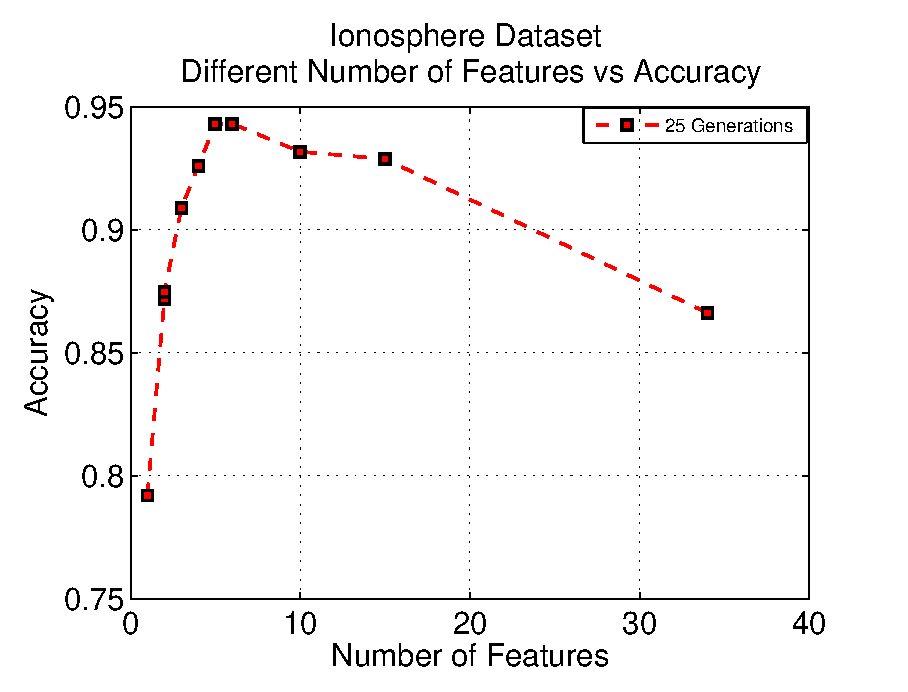
\includegraphics[width=0.6\linewidth]{img/ionfeat2.eps}
     \caption{Different Number of Features vs Accuracy}
    \end{figure}
    \begin{figure}[h!]
      \centering
      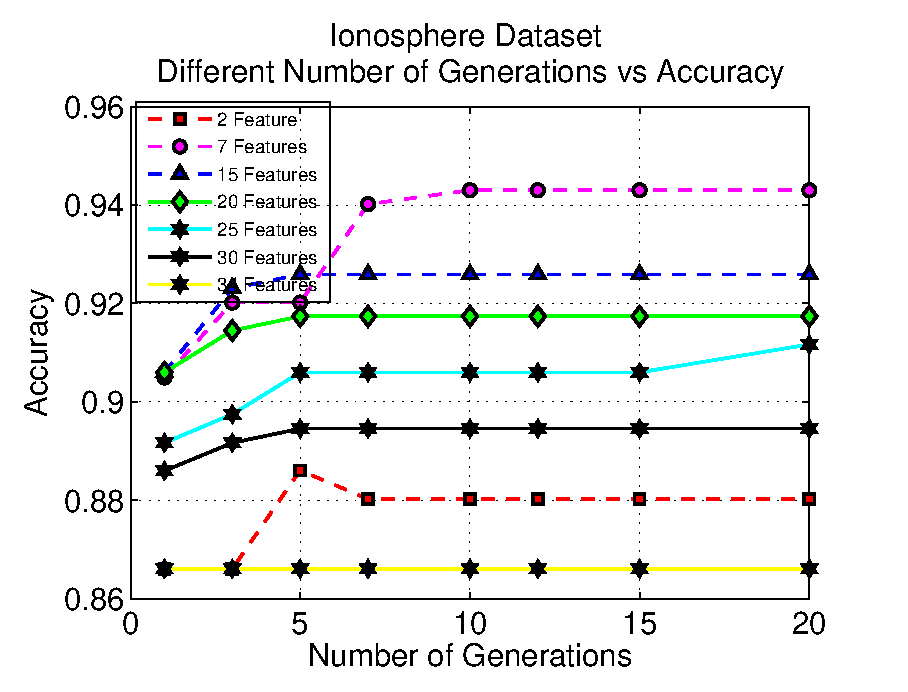
\includegraphics[width=0.6\linewidth]{img/ionfeat.eps}
      \caption{Different Number of Generations vs Accuracy}
    \end{figure}

Further testing performed was related to the observation of accuracy within the same number of features used but with varying the number of generations. In this experiment for the 2, 7, 15, 20, 25, 30, 35 numbers of features we varied the number of generation to 1, 3, 5, 7, 10, 15 and 20. For 1 feature taken, accuracy converges to 88\% after the 7th generation and remains identical till the 20th. For 7 features there is an increase between the 1st generations and the 5th from 90\% to 92.02\%. Also from the 7th generation onwards accuracy becomes stable acquiring the value of 94.3\%. For 15 features the same behaviour is observed with the accuracy increase from 1st generation till the 3rd from 90.6\% to 92.3\%. Above the 3rd generation the value remains the same. The same behaviour applies to the other number of features taken as shown in figure 2.
\begin{table}[ht]
\caption{Ionosphere Varying Features }
\resizebox{\textwidth}{!}{%
\begin{tabular}{|l|l|l|l|l|l|l|l|l|l|l|}
\hline
IONOSPHERE &  &  &  &  &  &  &  &  &  &  \\ \hline
(two class-problem, 34 features) & Run 1 & Run 2 & Run 3 & Run 4 & Run 5 & Run 6 & Run 7 & Run 8 & Run 9 & Run 10 \\ \hline
Features used & 1 & 2 & 2 & 3 & 4 & 5 & 6 & 10 & 15 & 34 \\ \hline
Crossover Rate & 0.6 & 0.6 & 0.6 & 0.6 & 0.6 & 0.6 & 0.6 & 0.6 & 0.6 & 0.6 \\ \hline
Mutation Rate & 0.01 & 0.01 & 0.1 & 0.1 & 0.1 & 0.1 & 0.1 & 0.1 & 0.1 & 0.1 \\ \hline
Generations & 25 & 25 & 25 & 25 & 25 & 25 & 25 & 25 & 25 & 25 \\ \hline
Population Size & 50 & 50 & 50 & 50 & 50 & 50 & 50 & 50 & 50 & 50 \\ \hline
KNN & 1 & 1 & 1 & 1 & 1 & 1 & 1 & 1 & 1 & 1 \\ \hline
Best Feature Subset (index starts at 0!) & 4 & 4.9 & 2.3 & 4,15,23 & 6,7,15,23 & 0,4,13,20,23 & 4,8,11,14,15,23 & 5|23|26|28|7|33|22|4|0|20 & 26|6|4|19|33|12|27|20|3|23|17|22|15|14|16| & all \\ \hline
Accuracy of this subset & 0.7920 & 0.8718 & 0.8746 & 0.9088 & 0.9259 & 0.9430 & 0.9430 & 0.9316 & 0.9287 & 0.8661 \\ \hline
\end{tabular}
}
\end{table}
Also from table 1 we could observe the subsets of solutions that are the optimal for each case.
\subsection{Semeion Handwritten Digit Dataset}

    \begin{figure}[ht!]
      \centering
      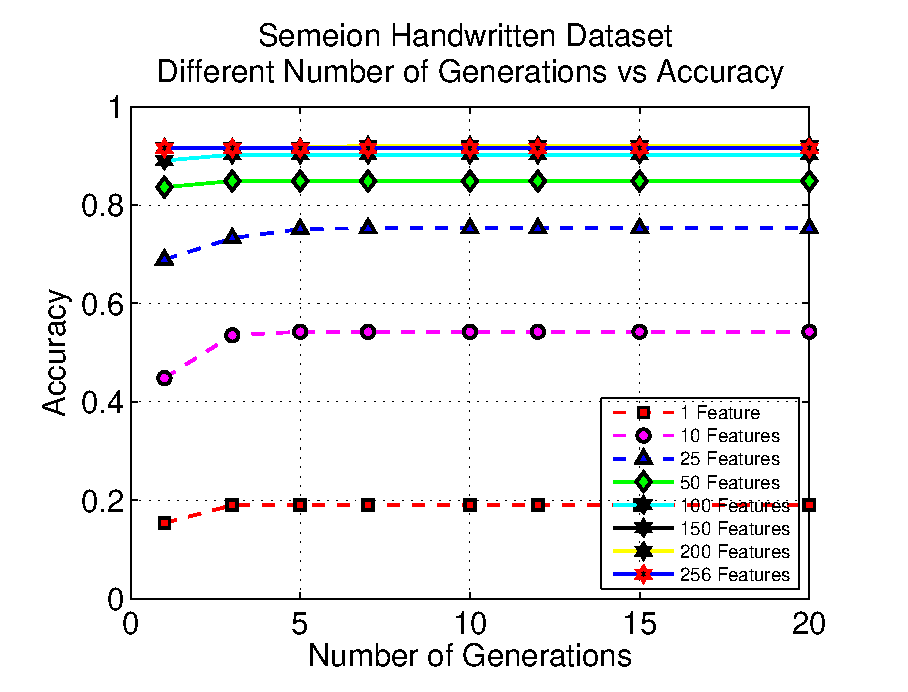
\includegraphics[width=0.6\linewidth]{img/seimfeat.eps}
      \caption{Different Number of Generations vs Accuracy}
    \end{figure}
    \begin{figure}[h!]
          \centering
          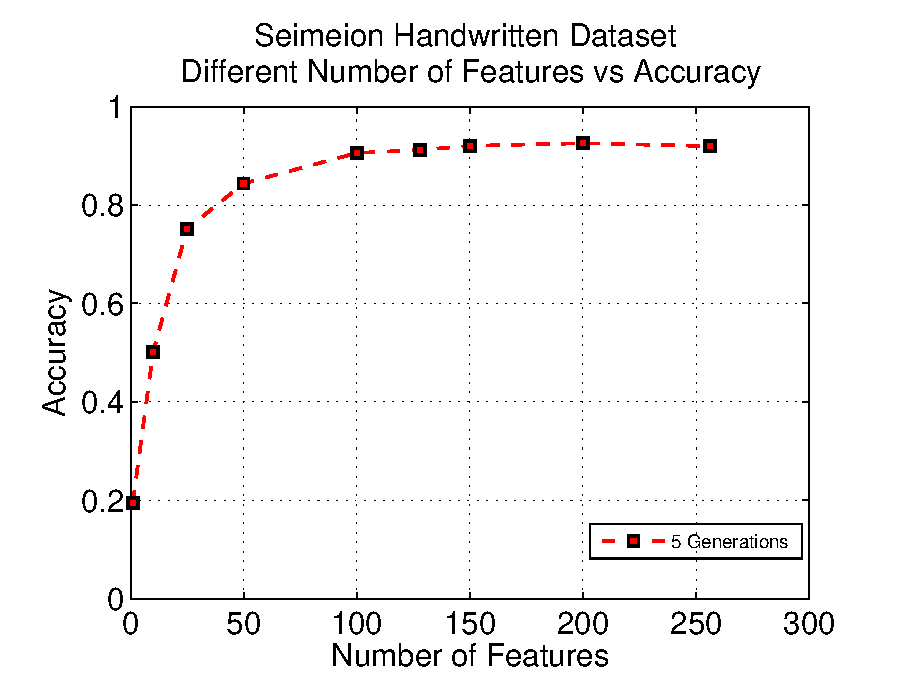
\includegraphics[width=0.6\linewidth]{img/seimfeat2.eps}
          \caption{Different Number of Features vs Accuracy}
    \end{figure}
        
Using the Semeion Handwritten Digit dataset a similar experiment was performed as with the previous database. Firstly it was observed that for considering all the 256 features taken from the 1st generation the accuracy remained the same for all different generations. When taking 200 the accuracy gets higher after the 3rd generation from 92.66\% to 92.78\% and remained identical for all the different generation up to the 20th. As taking lower features and particularly 150 features at the from the 1st till the 3rd iteration accuracy was of 91.59\% then at the 5th generation accuracy got higher to 91.65\% and finally settling to 92.03\%. This tendency was repeated for all the other resulting accuracies with their respective chosen features and predefined number of generations shown in figure 3. 

    
    
    
    Furthermore we have tested for the accuracy's behaviour within a number of generation and varying the selected features. The achieved accuracy was an outcome that was produced with a steady crossover rate of 0.6 and mutation rate of 0.1 with predefined 50 generations and a population of 50. Knn was also set to 1. The varying parameter in this measurement was the features used. We used for our test 1, 10, 25, 50, 100, 128, 150, 200 and 256 features and ran the code the respective 9 times. From figure 4 it was observed that the accuracy was increasing between the subset of 1 to 8 features taken reaching its peak accuracy of 92.53\% when 8 features were selected. Above 8 features and till 9 features the accuracy dropped to 91.96\%.    

\subsection{Red Wine Dataset }

  \begin{figure}[h!]
      \centering
      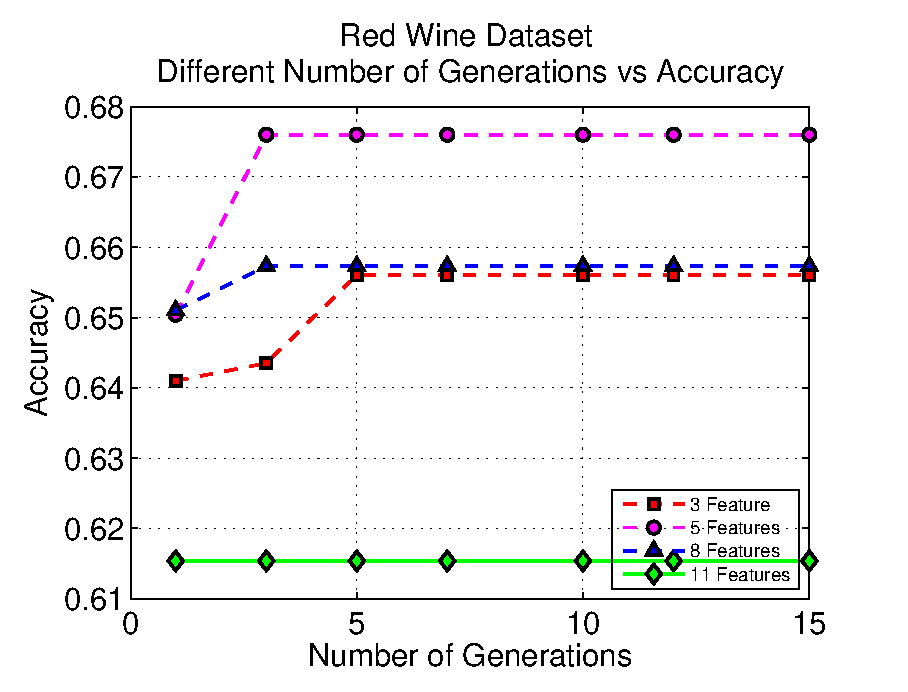
\includegraphics[width=0.6\linewidth]{img/winefeat.eps}
      \caption{Different Number of Generations vs Accuracy}
   \end{figure}
 In the red wine dataset the first step in testing was to vary the features taken with 3, 5, 8,1 1 and for every varying  feature different number of generation were used of 1, 3, 5, 7, 10, 12, and 15. This resulted for every number of features taken between the 1st and the 3rd generation the value of accuracy to become higher and then after the 3rd generation it remains stable till all the generations are taken into consideration. Only when taking 11 features, from the first generation till the 15th the value of accuracy remains the same as shown in figure 5.    
   
      \begin{figure}[h!]
        \centering
        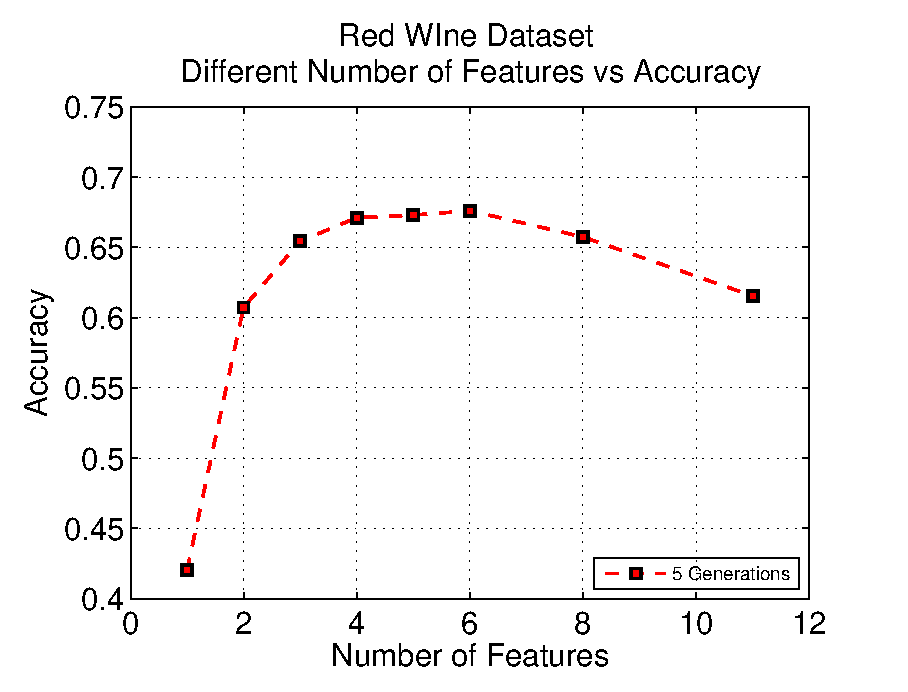
\includegraphics[width=0.6\linewidth]{img/winefeat2.eps}
       \caption{Different Number of Features vs Accuracy}
      \end{figure}
Finally, when evaluating the accuracy for a fixed number of 5 generators and varying number of features taken with 1, 2, 3, 4, 5, 6, 8, 11 features. Accuracy was rising from the 1st feature used with 42.03\% to 67.60\% with 6 features taken. Between 6 and 11 features, accuracy fall to 61.54\% figure 6.
   
   
   \begin{table}[t]
   \caption{Red Wine Varying Features}
   \resizebox{\textwidth}{!}{%
   \begin{tabular}{|l|l|l|l|l|l|l|l|l|}
   \hline
   (Red Wine Dataset) & Run 1 & Run 2 & Run 3 & Run 4 & Run 5 & Run 6 & Run 7 & Run 8 \\ \hline
   Features used & 1 & 2 & 3 & 4 & 5 & 6 & 8 & 11 \\ \hline
   Crossover Rate & 0.6 & 0.6 & 0.6 & 0.6 & 0.6 & 0.6 & 0.6 & 0.6 \\ \hline
   Mutation Rate & 0.1 & 0.1 & 0.1 & 0.1 & 0.1 & 0.1 & 0.1 & 0.1 \\ \hline
   Generations & 5 & 5 & 5 & 5 & 5 & 5 & 5 & 5 \\ \hline
   Population Size & 50 & 50 & 50 & 50 & 50 & 50 & 50 & 50 \\ \hline
   KNN & 1 & 1 & 1 & 1 & 1 & 1 & 1 & 1 \\ \hline
   Best Feature Subset (index starts at 0!) & 7 & 7|10 & 0|1|10 & 2|8|9|10 & 1|7|8|9|10 & 1|4|7|8|9|10 & 0|1|2|4|7|8|9|10 & all \\ \hline
   Accuracy of this subset & 0.4203 & 0.6072 & 0.6542 & 0.6710 & 0.6729 & 0.6760 & 0.6573 & 0.6154 \\ \hline
   \end{tabular}
   }
   \end{table}
From table 2, it could be observed that how the varying features are affecting the accuracy and their respective optimal subset of features solution.

 \begin{table}[ht]
 \caption{Red Wine Varying Generations, 3 Features}
 
 \resizebox{\textwidth}{!}{%
 \begin{tabular}{|l|l|l|l|l|l|l|l|}
 \hline
 RED WINE QUALITY &  &  &  &  &  &  &  \\ \hline
 (6 CLASS-PROBLEM, 11 features) & Run 1 & Run 2 & Run 3 & Run 4 & Run 5 & Run 6 & Run 7 \\ \hline
 Features used & 3 & 3 & 3 & 3 & 3 & 3 & 3 \\ \hline
 Generations & 1 & 3 & 5 & 7 & 10 & 12 & 15 \\ \hline
 Crossover Rate & 0.6 & 0.6 & 0.6 & 0.6 & 0.6 & 0.6 & 0.6 \\ \hline
 Mutation Rate & 0.1 & 0.1 & 0.1 & 0.1 & 0.1 & 0.1 & 0.1 \\ \hline
 Population Size & 50 & 50 & 50 & 50 & 50 & 50 & 50 \\ \hline
 KNN & 1 & 1 & 1 & 1 & 1 & 1 & 1 \\ \hline
 Accuracy of this subset & 0.641 & 0.6435 & 0.656 & 0.656 & 0.656 & 0.656 & 0.656 \\ \hline
 \end{tabular}
 }
 \end{table}
 In table 3 we could observe that with 3 features used and with different generation the resulting accuracy it does not change beyond the 5th generation and therefore remains stable.

\section{Conclusion}
Choosing the correct parameters in Evolutionary Algorithms plays significant role in the degree of accuracy. From the experiments we concluded that by setting the optimal parameters for the crossover ratio and the mutation ratio, the biggest attention falls in number of generation and the features selected. In terms of the features selected, we realised that declaring a high number of features does not necessarily give the best results in terms of accuracy. The same applies for declaring a very low amount of features. The number of generations plays a significant role in the accuracy estimation and also in terms of computational time we established that there is no need for extreme values of generations since for all the databases, accuracy was not changing after 3 or 5 generations.   




\newpage


{\small
\bibliographystyle{abbrv}
\bibliography{rev}
}

\end{document}